\section{Tipus de matrius}

\textbf{Definició:} Una \textbf{matriu} d'ordre $(m, n)$ és un conjunt de nombres reals disposats en $m$ files i $n$ columnes. Cada nombre rep el nom d'\textbf{element}:

\begin{equation}
A = \begin{pmatrix} a_{11} & a_{12} & a_{13} & \cdots & a_{1n} \\ a_{21} & a_{22} & a_{23} & \cdots & a_{2n} \\ \vdots & \vdots & \vdots & \ddots & \vdots \\ a_{m1} & a_{m2} & a_{m3} & \cdots & a_{mn} \end{pmatrix}
\end{equation}

Els dos subíndexs de cada element $a_{ij}$ indiquen la seva posició: $i$ és la fila i $j$ la columna. Notació alternativa: $A = (a_{ij})$ amb $i = 1, \ldots, m$ i $j = 1, \ldots, n$.

Els tipus principals de matrius són:

\begin{itemize}
\item \textbf{Matriu oposada} $(-A)$: s'obté canviant cada element pel seu oposat.
\item \textbf{Matriu transposada} $(A^t)$: resulta d'intercanviar files per columnes.
\item \textbf{Matriu identitat} $(I)$: matriu quadrada amb $a_{ij} = 1$ si $i = j$ i $a_{ij} = 0$ si $i \neq j$:
\end{itemize}

\begin{equation*}
I = \begin{pmatrix} 1 & 0 & 0 \\ 0 & 1 & 0 \\ 0 & 0 & 1 \end{pmatrix}
\end{equation*}

\begin{itemize}
\item \textbf{Matriu nul\textperiodcentered{}la:} tots els elements són $0$.
\end{itemize}

\section{Operacions amb matrius}

\subsection{Suma de matrius del mateix ordre}

Donades $A = (a_{ij})$ i $B = (b_{ij})$ del mateix ordre $(m, n)$:

\begin{equation*}
A + B = (a_{ij} + b_{ij})
\end{equation*}

Es sumen els elements que ocupen la mateixa posició.

\subsection{Producte d'un nombre real per una matriu}

Donat $k \in \mathbb{R}$ i $A = (a_{ij})$:

\begin{equation*}
k\cdot A = (k\,a_{ij})
\end{equation*}

\subsection{Producte de matrius}

Donades $A_{m\times n} = (a_{ij})$ i $B_{n\times p} = (b_{ij})$ (el nombre de columnes de $A$ ha de coincidir amb el de files de $B$), la matriu producte $C = A\cdot B$ és de tipus $m\times p$ amb:

\begin{equation*}
c_{ij} = \sum_{k=1}^{n} a_{ik}b_{kj} = a_{i1}b_{1j} + a_{i2}b_{2j} + \cdots + a_{in}b_{nj}
\end{equation*}

\emph{Observació:} en general, el producte de matrius \textbf{no és commutatiu}: $A\cdot B \neq B\cdot A$.

\subsection{Potència d'una matriu quadrada}

La potència enèsima d'una matriu quadrada $A$ és:

\begin{equation*}
A^n = A^{n-1}\cdot A, \qquad n \in \mathbb{N},\; n \ge 2
\end{equation*}

\section{Determinants}

Els determinants van associats a les matrius quadrades. El determinant de $A$ es simbolitza per $|A|$ o $\det(A)$.

\subsection{Determinant d'ordre 2}

\begin{equation*}
|A| = \begin{vmatrix} a_{11} & a_{12} \\ a_{21} & a_{22} \end{vmatrix} = a_{11}\cdot a_{22} - a_{12}\cdot a_{21}
\end{equation*}

\subsection{Determinant d'ordre 3. Regla de Sarrus}

\begin{equation*}
|A| = \begin{vmatrix} a_{11} & a_{12} & a_{13} \\ a_{21} & a_{22} & a_{23} \\ a_{31} & a_{32} & a_{33} \end{vmatrix} = a_{11}a_{22}a_{33} + a_{12}a_{23}a_{31} + a_{13}a_{21}a_{32} - a_{13}a_{22}a_{31} - a_{12}a_{21}a_{33} - a_{11}a_{23}a_{32}
\end{equation*}

La \textbf{regla de Sarrus} és un mètode gràfic per recordar aquesta fórmula: s'afegeixen les dues primeres columnes a la dreta de la matriu i s'identifiquen les sis diagonals (tres amb signe $+$ i tres amb signe $-$):

\begin{figure}[!htbp]
\centering
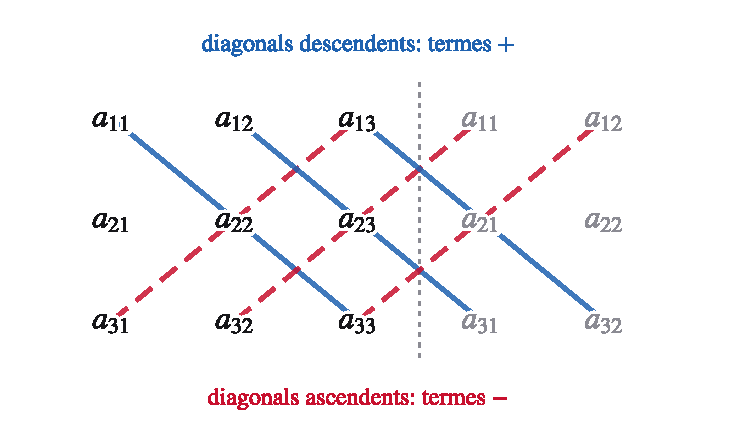
\includegraphics[width=353pt]{fig/m07_f16.pdf}
\caption{Regla de Sarrus: les tres diagonals descendents donen termes positius; les tres diagonals ascendents (en les columnes repetides), termes negatius.}
\end{figure}

\section{Adjunts d'una matriu quadrada}

D'una matriu qualsevol es poden extreure submatrius quadrades. Els determinants d'aquestes submatrius s'anomenen \textbf{menors} d'ordre $k$.

\textbf{Definició:} El \textbf{menor complementari} $M_{ij}$ és el determinant que resulta de suprimir la fila $i$ i la columna $j$ d'una matriu quadrada.

L'\textbf{adjunt} de l'element $(i, j)$ és:

\begin{equation*}
m_{ij} = (-1)^{i+j}\,M_{ij}
\end{equation*}

El signe $(-1)^{i+j}$ segueix el patró escaquer següent:

\begin{equation*}
\begin{pmatrix} + & - & + \\ - & + & - \\ + & - & + \end{pmatrix}
\end{equation*}

La \textbf{matriu adjunta} de $A$ és $A^* = (m_{ij})$, la matriu formada per tots els adjunts.

\section{Propietats dels determinants}

\begin{itemize}
\item Si una línia (fila o columna) és combinació lineal de les altres, el determinant és zero.
\item Si dues línies són iguals, el determinant és zero.
\item $\det(A) = \det(A^t)$ (el determinant és igual al de la transposada).
\item Si s'intercanvien dues línies, el determinant canvia de signe.
\item Si es multiplica una línia per $k$, el determinant queda multiplicat per $k$.
\item Un determinant amb una línia de zeros és zero.
\item $\det(I) = 1$.
\end{itemize}

\section{Rang d'una matriu}

\textbf{Definició:} El \textbf{rang} d'una matriu és l'ordre màxim dels seus menors no nuls, o equivalentment, el nombre màxim de files (o columnes) linealment independents.

Per calcular el rang d'una matriu $A$ de tipus $m\times n$:

\begin{enumerate}
\item S'identifica la dimensió màxima possible: $\operatorname{rang}(A) \le \min(m, n)$.
\item Es calcula el determinant de la submatriu quadrada d'ordre màxim:
\begin{itemize}
\item Si $\det \neq 0$: el rang és igual a aquest ordre màxim.
\item Si $\det = 0$: cal analitzar menors d'ordre inferior.
\end{itemize}
\item Es repeteix el procés reduint l'ordre fins trobar un menor no nul.
\end{enumerate}

\section{Matriu inversa}

\textbf{Definició:} La \textbf{matriu inversa} d'una matriu quadrada $A$ és la matriu $A^{-1}$ que verifica

\begin{equation}
A\cdot A^{-1} = A^{-1}\cdot A = I
\end{equation}

Una matriu que té inversa s'anomena \textbf{matriu regular}. Una matriu és regular si i només si $\det(A) \neq 0$.

La matriu inversa es calcula mitjançant la matriu adjunta transposada:

\begin{equation*}
A^{-1} = \frac{1}{|A|}\cdot(A^*)^t
\end{equation*}

\emph{Observació:} si $\det(A) = 0$, la matriu és \textbf{singular} i no té inversa.

\section{Complement: potències, equacions matricials i mètode de Gauss-Jordan}

\subsection{Potències d'una matriu: buscar el patró}

Per calcular $A^n$ amb $n$ gran no es multiplica $n$ vegades: es calculen $A^2,\,A^3,\dots$ fins veure un \textbf{patró} i es demostra per inducció.

\emph{Exemple:} $A=\begin{pmatrix}1&1\\0&1\end{pmatrix}$. Llavors $A^2=\begin{pmatrix}1&2\\0&1\end{pmatrix}$ i $A^3=\begin{pmatrix}1&3\\0&1\end{pmatrix}$, de manera que

\begin{equation*}
A^n=\begin{pmatrix}1&n\\0&1\end{pmatrix}
\end{equation*}

\emph{Demostració per inducció:} es compleix per a $n=1$; si és cert per a $n$, $A^{n+1}=A^n\cdot A=\begin{pmatrix}1&n\\0&1\end{pmatrix}\begin{pmatrix}1&1\\0&1\end{pmatrix}=\begin{pmatrix}1&n+1\\0&1\end{pmatrix}$.

\emph{Exemple (potències periòdiques):} Si $B=\begin{pmatrix}0&1\\-1&0\end{pmatrix}$, llavors $B^2=-I$, $B^3=-B$ i $B^4=I$. Les potències es repeteixen cada $4$: per a calcular $B^{2026}$ n'hi ha prou amb el residu de $2026$ entre $4$ (que és $2$), i per tant $B^{2026}=B^2=-I$.

\subsection{Equacions matricials}

Com que el producte de matrius \textbf{no és commutatiu}, cal aïllar $X$ multiplicant per la inversa \textbf{pel mateix costat} a tots dos membres:

\begin{table}[!htbp]
\centering
\renewcommand{\arraystretch}{1.3}
\begin{tabularx}{\textwidth}{l>{\raggedright\arraybackslash}X}
\toprule
Equació & Solució (si les matrius són invertibles) \\
\midrule
$A\,X=B$ & $X=A^{-1}B$ \\
$X\,A=B$ & $X=B\,A^{-1}$ \\
$A\,X+B=C$ & $X=A^{-1}(C-B)$ \\
$A\,X\,B=C$ & $X=A^{-1}\,C\,B^{-1}$ \\
$A\,X+X=B$ & $(A+I)\,X=B\Rightarrow X=(A+I)^{-1}B$ \\
\bottomrule
\end{tabularx}
\end{table}

\emph{Atenció:} en $A\,X+X=B$ no es pot treure ``factor comú'' sense la identitat: $X=I\,X$, per això surt $(A+I)$ i no $(A+1)$.

\emph{Exemple 1:} Resoleu $A\,X=B$ amb $A=\begin{pmatrix}1&2\\0&1\end{pmatrix}$ i $B=\begin{pmatrix}3&4\\1&2\end{pmatrix}$.

$|A|=1\neq0$ i $A^{-1}=\begin{pmatrix}1&-2\\0&1\end{pmatrix}$. Llavors

\begin{equation*}
X=A^{-1}B=\begin{pmatrix}1&-2\\0&1\end{pmatrix}\begin{pmatrix}3&4\\1&2\end{pmatrix}=\begin{pmatrix}1&0\\1&2\end{pmatrix}
\end{equation*}

\emph{Comprovació:} $A\,X=\begin{pmatrix}1+2&0+4\\1&2\end{pmatrix}=B$ $\checkmark$.

\emph{Exemple 2:} Resoleu $A\,X+X=B$ amb la mateixa $A$ i $B=\begin{pmatrix}2&4\\2&0\end{pmatrix}$.

$A+I=\begin{pmatrix}2&2\\0&2\end{pmatrix}$, amb $|A+I|=4$ i $(A+I)^{-1}=\dfrac14\begin{pmatrix}2&-2\\0&2\end{pmatrix}$.

\begin{equation*}
X=(A+I)^{-1}B=\frac14\begin{pmatrix}2&-2\\0&2\end{pmatrix}\begin{pmatrix}2&4\\2&0\end{pmatrix}=\frac14\begin{pmatrix}0&8\\4&0\end{pmatrix}=\begin{pmatrix}0&2\\1&0\end{pmatrix}
\end{equation*}

\emph{Exemple 3 (amb paràmetre):} Per a quins valors de $m$ té inversa $A=\begin{pmatrix}1&m\\2&3\end{pmatrix}$? Té inversa si i només si $|A|=3-2m\neq0$, és a dir, per a $m\neq\dfrac32$.

\subsection{Càlcul de la inversa pel mètode de Gauss-Jordan}

Alternativa a la fórmula dels adjunts, més còmoda per a matrius $3\times3$. S'escriu $(A\,|\,I)$ i, amb operacions entre files, es transforma $A$ en $I$; la part dreta es converteix en $A^{-1}$.

\emph{Exemple:} $A=\begin{pmatrix}2&1\\5&3\end{pmatrix}$:

\begin{equation*}
\left(\begin{array}{cc|cc}2&1&1&0\\5&3&0&1\end{array}\right)\xrightarrow{F_1/2}\left(\begin{array}{cc|cc}1&\frac12&\frac12&0\\5&3&0&1\end{array}\right)\xrightarrow{F_2-5F_1}\left(\begin{array}{cc|cc}1&\frac12&\frac12&0\\0&\frac12&-\frac52&1\end{array}\right)
\end{equation*}

\begin{equation*}
\xrightarrow{2F_2}\left(\begin{array}{cc|cc}1&\frac12&\frac12&0\\0&1&-5&2\end{array}\right)\xrightarrow{F_1-\frac12F_2}\left(\begin{array}{cc|cc}1&0&3&-1\\0&1&-5&2\end{array}\right)\;\Rightarrow\;A^{-1}=\begin{pmatrix}3&-1\\-5&2\end{pmatrix}
\end{equation*}

Si en algun moment apareix una fila de zeros a la part esquerra, $A$ \textbf{no té inversa}.

\section{Complement: interpretació geomètrica del determinant}

El valor absolut del determinant $2\times2$ és l'\textbf{àrea del paral\textperiodcentered{}lelogram} definit per les seves files (o columnes); el del determinant $3\times3$ és el \textbf{volum del paral\textperiodcentered{}lelepípede}.

\begin{figure}[!htbp]
\centering
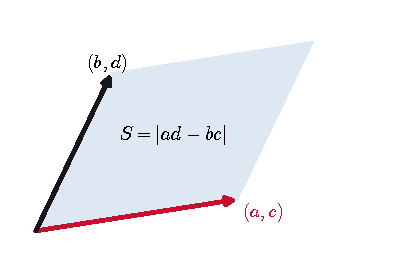
\includegraphics[width=194pt]{fig/x07_det_area.pdf}
\caption{El determinant de la matriu de columnes $(a,c)$ i $(b,d)$ és l'àrea (amb signe) del paral\textperiodcentered{}lelogram que formen.}
\end{figure}

\emph{Exemple:} Els vectors $(3,1)$ i $(1,2)$ determinen un paral\textperiodcentered{}lelogram d'àrea $\left|\begin{matrix}3&1\\1&2\end{matrix}\right|=6-1=5$.

Si $|A|=0$ els vectors són linealment dependents: el paral\textperiodcentered{}lelogram és ``pla'' (àrea $0$).

\section{Complement: propietats de la transposada i la inversa}

\begin{itemize}
\item $(A+B)^{t}=A^{t}+B^{t}$, $(kA)^{t}=kA^{t}$, $(AB)^{t}=B^{t}A^{t}$, $(A^{t})^{t}=A$.
\item $(AB)^{-1}=B^{-1}A^{-1}$, $(A^{-1})^{-1}=A$, $(A^{t})^{-1}=(A^{-1})^{t}$.
\item $|AB|=|A|\,|B|$, $|A^{t}|=|A|$, $|A^{-1}|=\dfrac1{|A|}$, $|kA|=k^{n}|A|$ si $A$ és d'ordre $n$.
\item Una matriu quadrada és \textbf{simètrica} si $A^{t}=A$ i \textbf{antisimètrica} si $A^{t}=-A$; és \textbf{ortogonal} si $A^{-1}=A^{t}$ (aleshores $|A|=\pm1$).
\item Una matriu quadrada té inversa si i només si $|A|\neq0$ si i només si $\operatorname{Rg}A=n$.
\item En general $AB\neq BA$; tampoc no es compleix $(A+B)^2=A^2+2AB+B^2$, sinó $(A+B)^2=A^2+AB+BA+B^2$.
\end{itemize}

\section{Complement: exemples resolts de determinants i inverses}

\emph{Exemple 1 --- Determinant amb paràmetre:} Per a quins valors de $a$ és invertible $A=\begin{pmatrix}1&1&1\\1&a&1\\1&1&a^2\end{pmatrix}$? Per Sarrus,

\begin{equation*}
|A|=a^3+1+1-a-a^2-1=a^3-a^2-a+1=(a-1)^2(a+1).
\end{equation*}

Així, $A$ és invertible si i només si $a\neq1$ i $a\neq-1$.

\emph{Exemple 2 --- Inversa per adjunts:} Sigui $B=\begin{pmatrix}1&0&2\\0&1&1\\1&1&0\end{pmatrix}$. Aleshores $|B|=-3\neq0$. Els adjunts són $B_{11}=-1$, $B_{12}=1$, $B_{13}=-1$, $B_{21}=2$, $B_{22}=-2$, $B_{23}=-1$, $B_{31}=-2$, $B_{32}=-1$, $B_{33}=1$. Per tant

\begin{equation*}
B^{-1}=\frac{1}{|B|}\bigl(\operatorname{Adj}B\bigr)^{t}=-\frac13\begin{pmatrix}-1&2&-2\\1&-2&-1\\-1&-1&1\end{pmatrix}=\begin{pmatrix}\frac13&-\frac23&\frac23\\-\frac13&\frac23&\frac13\\\frac13&\frac13&-\frac13\end{pmatrix}.
\end{equation*}

Es comprova que $B\,B^{-1}=I$ multiplicant.

\emph{Exemple 3 --- Rang amb paràmetre:} $\operatorname{Rg}\begin{pmatrix}1&2&3\\2&4&m\end{pmatrix}$: el menor $\begin{vmatrix}1&2\\2&4\end{vmatrix}=0$; amb la tercera columna, $\begin{vmatrix}1&3\\2&m\end{vmatrix}=m-6$. Si $m=6$, $\operatorname{Rg}=1$; si $m\neq6$, $\operatorname{Rg}=2$.

\emph{Exemple 4 --- Potència d'una matriu:} Per a $A=\begin{pmatrix}1&1\\0&1\end{pmatrix}$, $A^2=\begin{pmatrix}1&2\\0&1\end{pmatrix}$, $A^3=\begin{pmatrix}1&3\\0&1\end{pmatrix}$ i, per inducció, $A^n=\begin{pmatrix}1&n\\0&1\end{pmatrix}$.

\section{Complement: càlcul pràctic de determinants}

\subsection{Desenvolupament per una fila o columna (Laplace)}

El determinant d'una matriu quadrada és la suma dels elements d'una fila (o columna) multiplicats pels seus \textbf{adjunts}:

\begin{equation*}
|A|=\sum_{j=1}^{n}a_{ij}A_{ij},\qquad A_{ij}=(-1)^{i+j}M_{ij},
\end{equation*}

on $M_{ij}$ és el determinant que resulta d'esborrar la fila $i$ i la columna $j$. Convé triar la fila o columna amb més zeros. Els signes $(-1)^{i+j}$ formen un tauler d'escacs que comença amb $+$ a dalt a l'esquerra.

\emph{Exemple:} Calculem $\begin{vmatrix}2&0&0&1\\1&3&0&0\\0&1&1&2\\1&0&2&1\end{vmatrix}$ desenvolupant per la primera fila:

\begin{equation*}
=2\begin{vmatrix}3&0&0\\1&1&2\\0&2&1\end{vmatrix}-1\begin{vmatrix}1&3&0\\0&1&1\\1&0&2\end{vmatrix}=2\,(3\cdot(1-4))-5=-18-5=-23.
\end{equation*}

El signe de l'element $a_{14}$ és $(-1)^{1+4}=-1$.

\subsection{Triangularització (Gauss)}

Si una matriu és \textbf{triangular} (tots els elements per sota, o per sobre, de la diagonal són zero), el seu determinant és el \textbf{producte dels elements de la diagonal}. Per triangularitzar es poden fer aquestes operacions:

\begin{table}[!htbp]
\centering
\renewcommand{\arraystretch}{1.3}
\begin{tabularx}{\textwidth}{>{\raggedright\arraybackslash}X>{\raggedright\arraybackslash}X}
\toprule
Operació & Efecte sobre el determinant \\
\midrule
Intercanviar dues files (o columnes) & canvia de signe \\
Multiplicar una fila per $k\neq0$ & el determinant queda multiplicat per $k$ \\
Sumar a una fila un múltiple d'una altra ($F_i\to F_i+\lambda F_j$) & \textbf{no canvia} \\
\bottomrule
\end{tabularx}
\caption{Operacions elementals i determinant}
\end{table}

\emph{Exemple:} $\begin{vmatrix}1&2&1\\2&-1&1\\3&1&-2\end{vmatrix}$: fent $F_2\to F_2-2F_1$ i $F_3\to F_3-3F_1$ s'obté $\begin{vmatrix}1&2&1\\0&-5&-1\\0&-5&-5\end{vmatrix}$. Amb $F_3\to F_3-F_2$ queda $\begin{vmatrix}1&2&1\\0&-5&-1\\0&0&-4\end{vmatrix}=1\cdot(-5)\cdot(-4)=20$.

\subsection{Determinant de Vandermonde}

\begin{equation*}
\begin{vmatrix}1&1&1\\a&b&c\\a^{2}&b^{2}&c^{2}\end{vmatrix}=(b-a)(c-a)(c-b).
\end{equation*}

És diferent de zero si i només si $a$, $b$ i $c$ són tots diferents. Es demostra restant la primera columna a les altres dues i traient factor comú $(b-a)$ i $(c-a)$.

\section{Complement: rang d'una matriu pel mètode de Gauss}

Calcular el rang amb menors pot ser llarg. Un camí més ràpid és \textbf{escalonar} la matriu amb operacions entre files (que no canvien el rang): el rang és el nombre de \textbf{files no nul\textperiodcentered{}les} de la matriu escalonada.

\emph{Exemple:} $A=\begin{pmatrix}1&2&-1&3\\2&4&1&0\\3&6&0&3\end{pmatrix}$. Fent $F_2\to F_2-2F_1$ i $F_3\to F_3-3F_1$:

\begin{equation*}
\begin{pmatrix}1&2&-1&3\\0&0&3&-6\\0&0&3&-6\end{pmatrix}\xrightarrow{F_3\to F_3-F_2}\begin{pmatrix}1&2&-1&3\\0&0&3&-6\\0&0&0&0\end{pmatrix}.
\end{equation*}

Hi ha dues files no nul\textperiodcentered{}les: $\operatorname{Rg}A=2$.

\textbf{Propietats útils del rang.}

\begin{itemize}
\item $\operatorname{Rg}A=\operatorname{Rg}A^{t}$ i $\operatorname{Rg}(A)\le\min(m,n)$.
\item Si es fa una fila de zeros, o una fila és combinació lineal de les altres, el rang baixa.
\item Una matriu quadrada d'ordre $n$ té rang $n$ si i només si $|A|\neq0$.
\item $\operatorname{Rg}(AB)\le\min\bigl(\operatorname{Rg}A,\operatorname{Rg}B\bigr)$.
\end{itemize}

\section{Complement: equacions matricials i problemes tipus PAU}

\subsection{Equacions matricials}

Per aïllar la incògnita $X$ cal recordar que el producte \textbf{no és commutatiu}: la inversa s'ha de multiplicar pel \textbf{mateix costat} a tots dos membres.

\begin{table}[!htbp]
\centering
\renewcommand{\arraystretch}{1.3}
\begin{tabularx}{\textwidth}{l>{\raggedright\arraybackslash}X}
\toprule
Equació & Solució (si $A$ és invertible) \\
\midrule
$AX=B$ & $X=A^{-1}B$ \\
$XA=B$ & $X=BA^{-1}$ \\
$AXB=C$ & $X=A^{-1}CB^{-1}$ \\
$AX+B=C$ & $X=A^{-1}(C-B)$ \\
$AX+X=B$ & $X=(A+I)^{-1}B$ \\
\bottomrule
\end{tabularx}
\caption{Equacions matricials habituals}
\end{table}

\emph{Exemple:} Resolem $AX+B=C$ amb $A=\begin{pmatrix}2&1\\1&1\end{pmatrix}$, $B=\begin{pmatrix}1&0\\2&3\end{pmatrix}$ i $C=\begin{pmatrix}5&1\\3&2\end{pmatrix}$. Com que $|A|=1$, $A^{-1}=\begin{pmatrix}1&-1\\-1&2\end{pmatrix}$ i

\begin{equation*}
X=A^{-1}(C-B)=\begin{pmatrix}1&-1\\-1&2\end{pmatrix}\begin{pmatrix}4&1\\1&-1\end{pmatrix}=\begin{pmatrix}3&2\\-2&-3\end{pmatrix}.
\end{equation*}

\subsection{Matrius especials}

\begin{itemize}
\item \textbf{Idempotent:} $A^{2}=A$. Per exemple $A=\begin{pmatrix}2&-2\\1&-1\end{pmatrix}$. Si és invertible només pot ser $A=I$.
\item \textbf{Involutiva:} $A^{2}=I$, és a dir, $A^{-1}=A$.
\item \textbf{Nilpotent:} $A^{k}=O$ per a algun $k$. Per exemple $\begin{pmatrix}0&1\\0&0\end{pmatrix}^{2}=O$. Cap matriu nilpotent no és invertible.
\item \textbf{Ortogonal:} $A^{-1}=A^{t}$; aleshores $|A|=\pm1$.
\end{itemize}

\emph{Exemple (tipus PAU):} Si $A^{2}-3A+2I=O$, aleshores $A$ és invertible i $A^{-1}=\tfrac12(3I-A)$. En efecte, $A(3I-A)=3A-A^{2}=2I$.

\subsection{Resum de mètodes}

\begin{table}[!htbp]
\centering
\renewcommand{\arraystretch}{1.75}
\begin{tabularx}{\textwidth}{>{\raggedright\arraybackslash}Xc}
\toprule
Vull\ldots{} & Mètode \\
\midrule
saber si $A$ és invertible & $|A|\neq0$ \\
calcular $A^{-1}$ ($2\times2$ o $3\times3$) & adjunts: $\displaystyle \frac{1}{|A|}(\operatorname{Adj}A)^{t}$ \\
calcular $A^{-1}$ (ordre $\ge3$) & Gauss--Jordan $(A\,|\,I)\to(I\,|\,A^{-1})$ \\
el rang d'una matriu petita & menors \\
el rang d'una matriu gran o amb paràmetres & escalonar \\
el determinant d'ordre $\ge4$ & Laplace o triangularitzar \\
\bottomrule
\end{tabularx}
\caption{Quin mètode triar}
\end{table}
